Our approach consists of three stages: (1) synthetic data generation with emotion-rich teacher responses, (2) acoustic feature extraction, and (3) emotion-conditioned student model training. Figure \ref{fig:architecture} illustrates the complete pipeline.

\begin{figure*}[t]
\centering
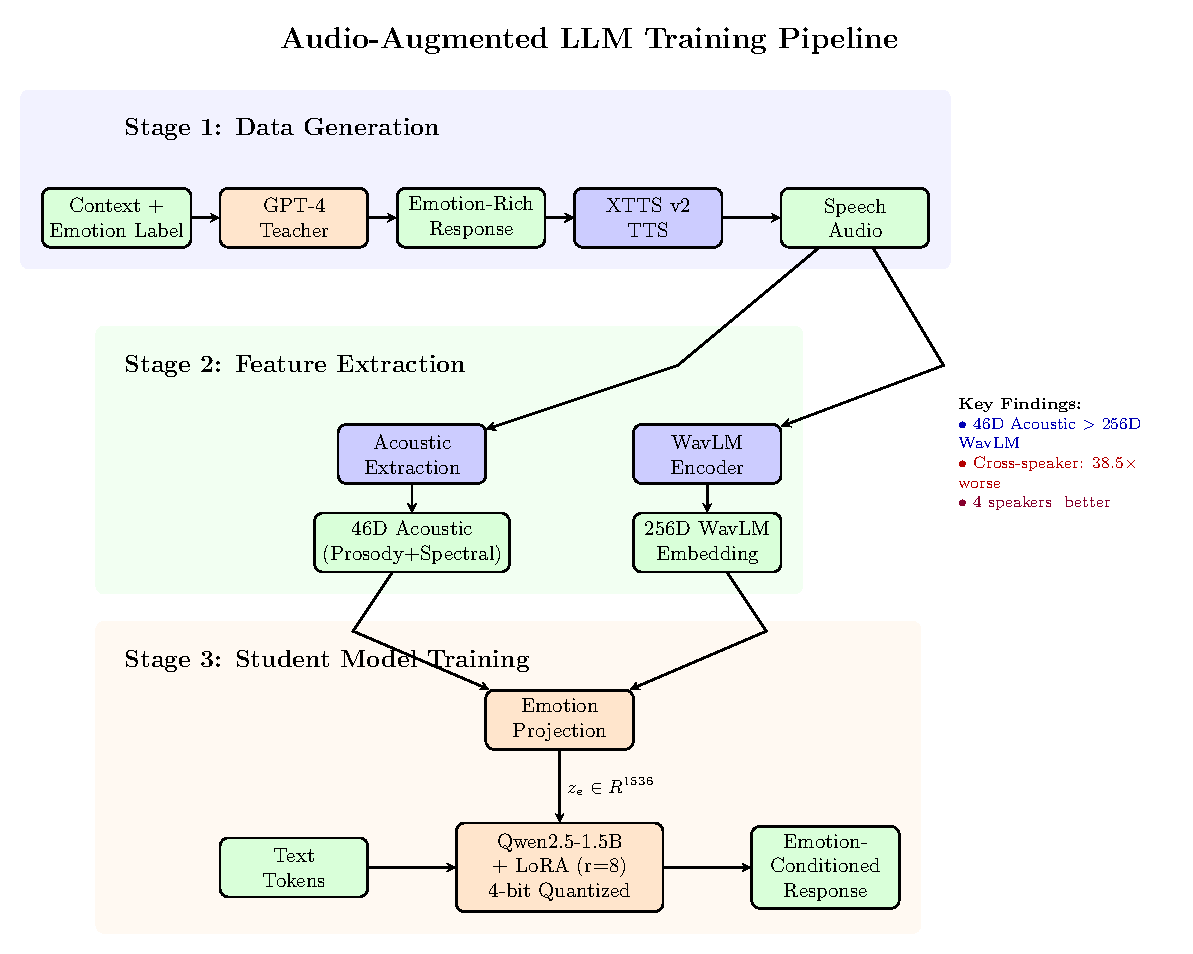
\includegraphics[width=0.95\textwidth]{figures/architecture.pdf}
\caption{System architecture for audio-augmented LLM training. The pipeline consists of three stages: (1) Data Generation using GPT-4 teacher and XTTS v2 TTS, (2) Feature Extraction using either acoustic features (46D) or WavLM embeddings (256D), and (3) Student Training with emotion projection and LoRA-adapted Qwen2.5-1.5B. Key findings highlight that compact acoustic features outperform deep embeddings for in-domain tasks, but cross-speaker generalization remains a critical challenge (38.5× performance degradation).}
\label{fig:architecture}
\end{figure*}

\subsection{Data Generation Pipeline}

\textbf{Teacher Response Generation.} We use a large language model (GPT-4) as a teacher to generate emotionally appropriate responses to conversational contexts. Given a context $c$ and target emotion $e \in \{\text{joy, anger, sadness, neutral, fear}\}$, we prompt the teacher:

\begin{quote}
\textit{``Generate a response expressing [emotion] to the context: [context]''}
\end{quote}

This produces emotion-labeled text pairs $(c, r_e)$ where $r_e$ is the teacher's response with emotion $e$.

\textbf{Text-to-Speech Synthesis.} We convert text responses to audio using XTTS v2 \cite{casanova2022xtts}, a state-of-the-art TTS model capable of high-quality emotional speech synthesis. This yields audio samples $a_e = \text{TTS}(r_e, \text{speaker})$ with prosodic patterns corresponding to the target emotion.

\subsection{Acoustic Feature Extraction}

We extract a 46-dimensional acoustic feature vector from each audio sample, organized into three groups:

\textbf{Prosodic Features (13D):} 
\begin{itemize}
    \item Pitch statistics: mean $\mu_{\text{F0}}$, std $\sigma_{\text{F0}}$, range, CV
    \item Energy statistics: mean $\mu_E$, std $\sigma_E$, range, CV  
    \item Speaking rate: syllables per second
    \item Voice quality: jitter, shimmer, HNR, ZCR
\end{itemize}

\textbf{Spectral Features (20D):}
\begin{itemize}
    \item MFCCs 1-13: spectral envelope characteristics
    \item Spectral statistics: centroid, bandwidth, rolloff, contrast
    \item Formants F1-F3: vocal tract resonances
\end{itemize}

\textbf{Formant Features (13D):}
\begin{itemize}
    \item Formant frequencies F1-F3 (mean, std, range, CV)
    \item Formant bandwidth (mean)
\end{itemize}

For comparison, we also extract WavLM embeddings \cite{chen2022wavlm}: 
$$h_{\text{WavLM}} = \text{WavLM}(a_e) \in \mathbb{R}^{256}$$

\subsection{Student Model Architecture}

\textbf{Base Model.} We use Qwen2.5-1.5B \cite{qwen2023} as our base LLM, chosen for its strong performance and moderate size suitable for parameter-efficient fine-tuning.

\textbf{Emotion Integration.} Given acoustic features $f_e \in \mathbb{R}^d$ and text input $x$, we project emotion features to the LLM's hidden dimension:
$$z_e = W_{\text{proj}} f_e + b_{\text{proj}} \in \mathbb{R}^{h}$$

We concatenate $z_e$ with text token embeddings:
$$h = [z_e; \text{Embed}(x)] \in \mathbb{R}^{(1+|x|) \times h}$$

The LLM then generates conditioned on this augmented input:
$$p(y | x, f_e) = \text{LLM}(h)$$

\textbf{Parameter-Efficient Training.} We employ LoRA \cite{hu2021lora} with rank $r=8$ and 4-bit quantization to enable efficient fine-tuning on limited hardware. Only the LoRA adapters and emotion projection layer are trainable, keeping the base model frozen.

\subsection{Training Objective}

We minimize standard language modeling loss:
$$\mathcal{L} = -\sum_{t=1}^{|y|} \log p(y_t | y_{<t}, x, f_e)$$

where $y$ is the teacher's emotion-labeled response.
